% I use a custom document class that can be found at
% github.com/mwhittaker/texmf. Honestly, it's a big pain in the butt to set it
% up. Sorry this document isn't easier to compile! If you have the hw document
% class set up, you can compile this document with `latexmk -pdf answers.tex`

\documentclass{hw}
\title{CS 5220 -- 2015-08-27 Preclass Questions}
\hypersetup{
  colorlinks = true,
  allcolors = blue,
}

\begin{document}
\maketitle{}

\begin{enumerate}
  \item
    Refer to \figref{speedup} and \figref{efficiency}. These plots were
    generated by \texttt{amdahl.py}.

  \item
    We have a central server serially processing and sending a set of tasks
    $\set{t_1, t_2, \ldots}$ to $p$ workers $\set{w_1, w_2, \ldots, w_p}$.
    Assume that the server sends task $t_i$ to worker $w_{i \bmod p}$. For
    example, if we had three workers, then the central server would send $t_1$
    to $w_1$, $t_2$ to $w_2$, $t_3$ to $w_3$, $t_4$ to $w_1$, $t_5$ to $w_2$,
    etc. Also assume that each worker has a task buffer such that the central
    server can send a task to a worker even if it is already working on a task.
    Now, consider the possible values of $\alpha$.

    \newcommand{\caseone}{\alpha \geq \frac{\tau}{p}}
    \newcommand{\casetwo}{\alpha < \frac{\tau}{p}}
    \begin{itemize}
      \item Case 1: $\caseone{}$. At time $\alpha$, $w_1$ receives $t_1$.
        Then at time $\alpha + p\alpha$, $w_1$ receives $t_{p + 1}$. If
        $\caseone{}$, then $p\alpha \geq \tau$, so between time $\alpha$ and
        time $\alpha + p\alpha$, $w_1$ has completed $t_1$. It then sits idle
        until it receives $t_{p + 1}$, at which point it immediately starts
        working. Here, the central server is the bottle neck, so the throughput
        of the program is bounded from above by $\cbox{\frac{1}{\alpha}}$.
      \item Case 2: $\casetwo{}$. As before, $w_1$ receives $t_1$ at time
        $\alpha$. At time $\alpha + p\alpha$, the central server sends task
        $t_{p + 1}$ to $w_1$. Since $\casetwo{}$, $w_1$ is still processing
        $t_1$ at time $\alpha + p\alpha$, so $t_{p + 1}$ is queued in the task
        buffer of $w_1$. $w_1$ will continue to work on $t_1$ until it finishes
        at which point it will \emph{immediately} begin work in item $t_{p +
        1}$. Here, the $p$ workers are the bottleneck, so the throughput of the
        program is bounded from above by somewhere between
        $\cbox{\frac{1}{\tau}~\text{to}~\frac{p}{\tau}}$.
    \end{itemize}

  \item You should not tune a piece of code if
    \begin{itemize}
      \item the time taken to tune the code is greater than the time gained
        from tuning,
      \item the tuning significantly decreases the readability or
        maintainability of the code, or
      \item the code you're tuning isn't a bottleneck of the program.
    \end{itemize}

  \item According to
    \href{http://www.intel.com/content/www/us/en/benchmarks/server/xeon-phi/xeon-phi-theoretical-maximums.html}{this
    intel spec sheet}, each Xeon Phi board runs a theoretical maximum of 1,011
    GFLOPS. With 15 such boards, we get $15 \times 1,011 = 15.165$ TFLOPS.

  \item
    I have four Intel Core i5-4210U CPUs each running at 1.70GHz. According to
    \href{http://stackoverflow.com/a/15657772/3187068}{this StackOverflow
    answer}, each processor can perform 4 double precision floating operations
    per second for a total of $4 \times 4 \times 1.7 = 27.2$ GFLOPS.
\end{enumerate}

\begin{figure}[h]
  \centering
  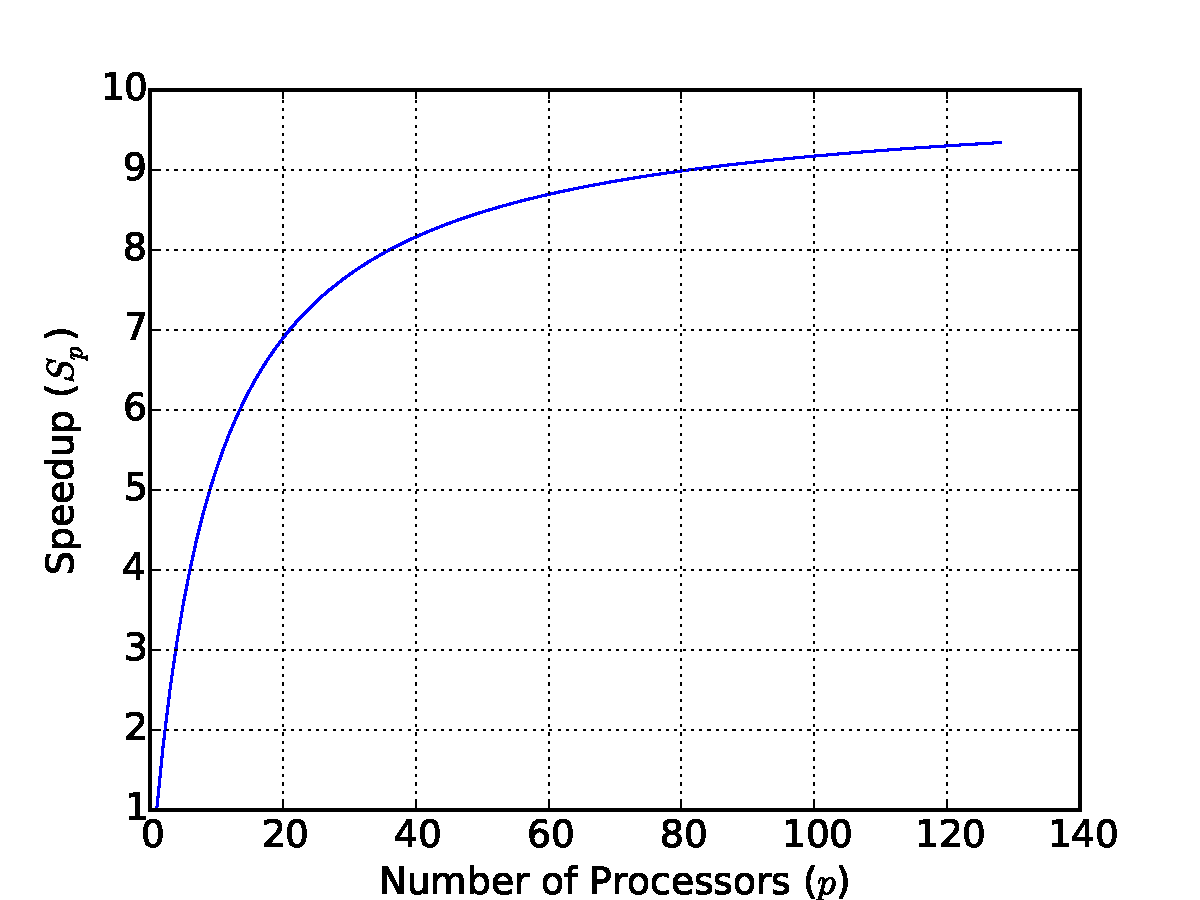
\includegraphics[width=\textwidth]{speedup.pdf}
  \caption{Speedup according to Amdahl's Law}
  \label{fig:speedup}
\end{figure}
\begin{figure}[h]
  \centering
  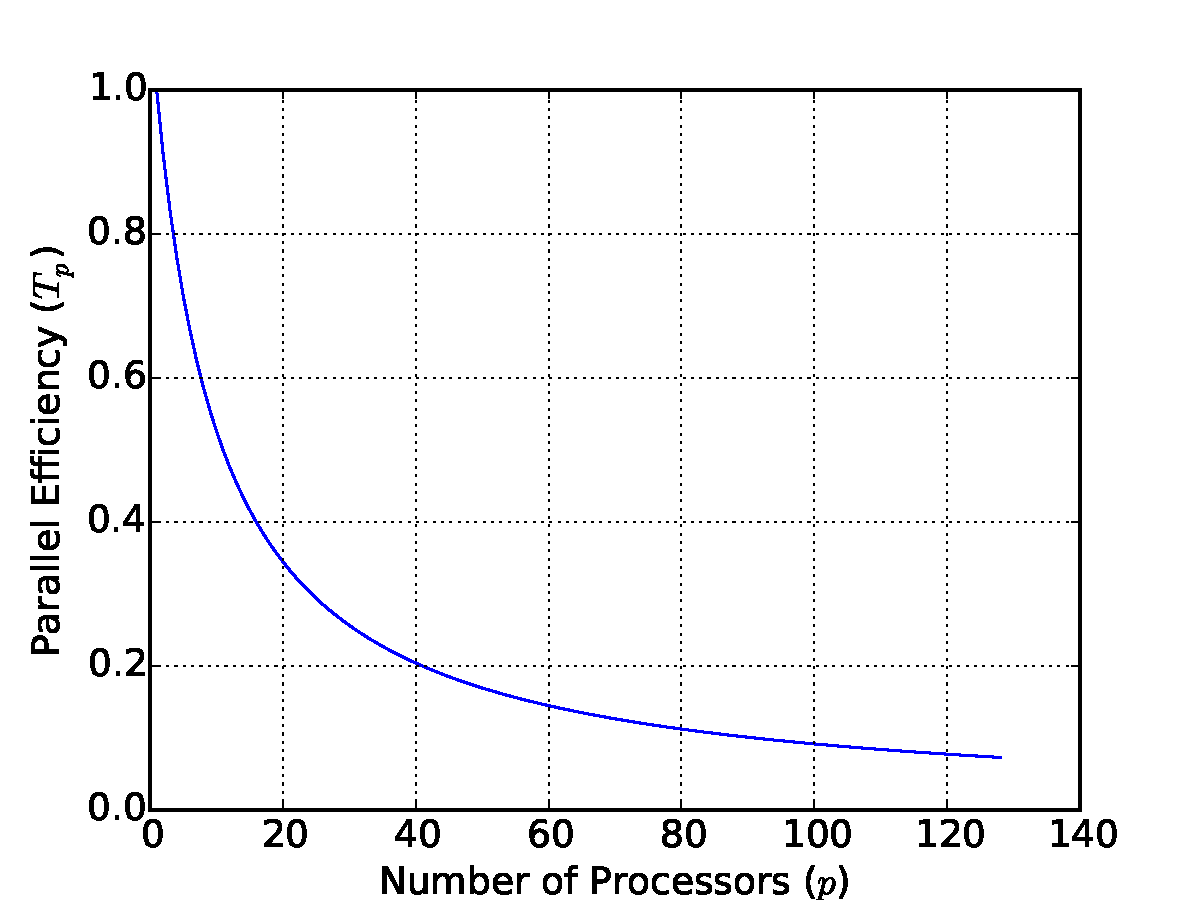
\includegraphics[width=\textwidth]{efficiency.pdf}
  \caption{Parallel efficiency according to Amdahl's Law}
  \label{fig:efficiency}
\end{figure}
\end{document}
